

\subsection{The DSLTrans Transformation Language}

% DSLTrans: why it was used to prove properties.
DSLTrans~\cite{Barroca2011} is an MTL used to specify model translations.
Its main distinctive feature is that the model translations that are described
in DSLTrans are guaranteed to always\markus{Where has this been shown?
Reference?} terminate\footnote{This result assumes that finite models are
used.}. This feature comes at a cost: DSLTrans is not Turing complete, i.e., no
unbounded recursion, non-determinist\markus{Is this sentence complete?} or
element deletion can be specified.
Despite the apparent lack of expressivity, our experience has showed that it is
possible to specify a wide range of transformations using DSLTrans. Furthermore,
it makes DSLTrans transformations ideal to prove properties about since the set
of possible behaviors is finite.

%Why use the families to persons example.
To present the syntax and semantics of DSLTrans, we will be using the Families-to-Persons transformation from the ATL transformation zoo \footnote{\url{http://www.eclipse.org/atl/atlTransformations}}.
Because this transformation can be easily understood, it allows us to focus on the essential concepts of DSLTrans.

%Metamodels of families to persons
Figure~\ref{fig:families_to_persons_metamodels} shows the metamodel of the Family language on the left, and the Community language on the right.
These two languages represent different perspectives of groups of people. A family has a father, mother, daughters and sons.
A community is composed of people and each person can either be a man or a woman.

\begin{figure}
        \centering
        \begin{subfigure}{0.5\linewidth}
                \centering
                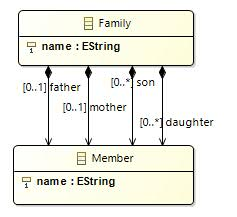
\includegraphics[width=\linewidth]{figures/Familiesclassdiagram}
                \caption{Families metamodel.}
                \label{fig:families_mm}
        \end{subfigure}%
        \begin{subfigure}{0.5\linewidth}
                \centering
                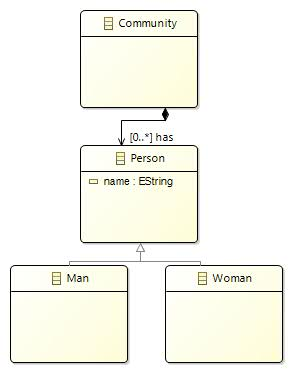
\includegraphics[width=\linewidth]{figures/communitydiagram}
                \caption{Community metamodel.}
                \label{fig:community_mm}
        \end{subfigure}%
        \caption{ }
        \label{fig:families_to_persons_metamodels}
\end{figure}

% Informal description of DSLTrans.
The partial translation of a family model into a community model, in DSLTrans,
is done by executing the transformation shown in
Figure~\ref{fig:families_mm}\markus{Figure is too small; font unreadable.}.
We show the partial transformation because it is sufficient to explain DSLTrans
semantics. DSLTrans transformations are organized in partial\markus{ly?} ordered
layers.
Each layer is executed after its previous layer. Each layer has a set of rules.
The execution of a layer means the execution of the rules that comprise that
layer.
The rules inside the same layer are executed independently of one another, i.e.,
there is no order of execution of rules and they cannot affect the execution
(e.g., enable or disable) of one another. Each rule has a \emph{match} pattern and an \emph{apply} pattern.
In Figure~\ref{fig:families_mm}, besides the input model description on the top,
there are two layers. The input model description contains the location of the
input model to be translated, which in this example is a family model. The first layer has two rules and the second layer
has one rule:
\begin{compactdesc}
	\item[FamilyRule] Find all the instances of Family and, for each one, create a Community element.
	\item[SonRule] Let $S = \left\{ (f, m_1) , \ldots , (f, m_n) \right\}$ be all instances, in the input model, of Family that are connected to instances of Member by the ``son'' association. This rule states that for each of those connected elements
$(f, m_i)$, create a Man element with a name defined by the concatenation of the name attribute of $m_i$ with the name attribute of $f$. Basically, it creates a man for each family member that is a son.
	\item[UnionManRule] \markus{In the Fig it is called UnionSonRUle} Let $S =
	\left\{ (f, m_1) , \ldots , (f, m_n) \right\}$ be all instances of Family that are connected to instances of Member by the ``son'' association.
	Now, let $R$ be the set formed by iterating each element $(f, m_i)$, finding
	the instance of Man ${man}_i$ that was created previously in SonRule and
	finding the instance $c$ of Community that was created in the FamilyRule. This
	rule iterates each element $(f, c, m_i, {man}_i)$ of the $R$ set and creates a
	``has'' association between $c$ and ${man}_i$. The trace\markus{Where do they
	come from?} links are of paramount importance to connect the instances created
	in rules of the \emph{previous} layer.
\end{compactdesc}

\begin{figure}
\begin{center}
  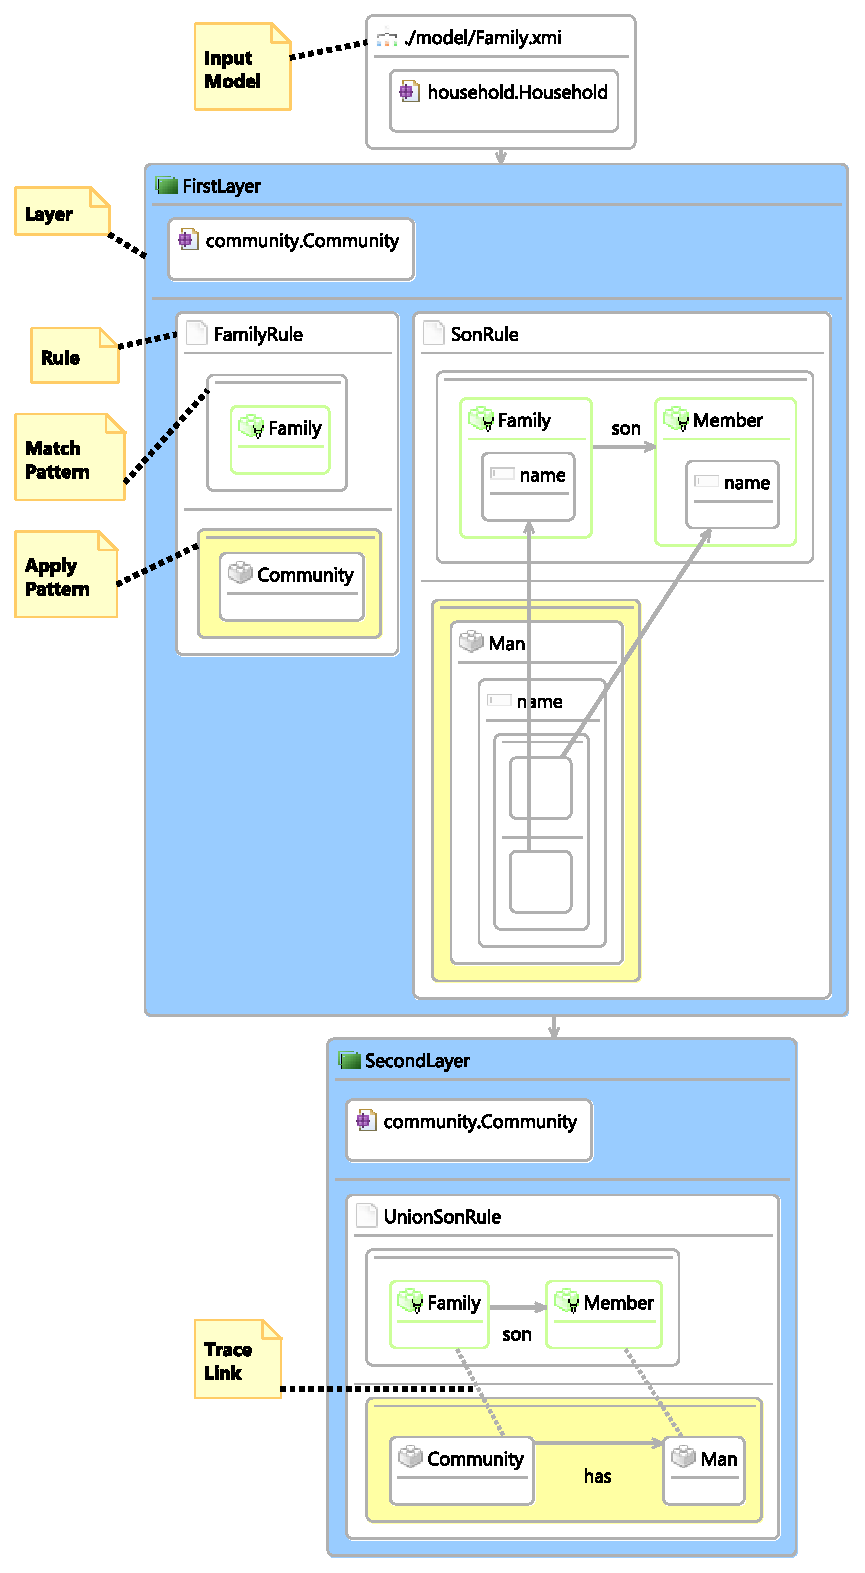
\includegraphics[width=0.35\textwidth]{figures/families_to_persons_hot2}
  \caption{DSLTrans transformation of Families to Communities (partial).}
  \label{fig:families_mm}
\end{center}
\end{figure}

% summary and bridge to the next section
In summary, if we apply the DSLTrans transformation partially shown in 
Figure~\ref{fig:families_mm} to a family model with a father, a mother, a son
and a daughter, we expect to get a community model with 2 men and 2 women. The
previous sentence represents a property about the transformation that we might
wish to verify automatically\markus{Really? Would a verification actually talk
about 2 men and 2 women? Wouldn't it be more general?}.


